\documentclass[aspectratio=169,10pt]{beamer}

\usepackage[utf8]{inputenc}
\usepackage{amsmath, amssymb}
\usepackage{xcolor}
\usepackage{tikz}
\usetikzlibrary{arrows.meta, positioning, shapes.geometric}
\usepackage{graphicx}

\usetheme{metropolis}

\definecolor{navymain}{RGB}{26, 43, 76}
\definecolor{navylight}{RGB}{200, 210, 225}
\definecolor{accentred}{RGB}{180, 60, 60}
\definecolor{winner}{RGB}{30, 110, 60}
\definecolor{gray60}{RGB}{120, 128, 140}

\setbeamercolor{frametitle}{bg=navymain, fg=white}
\setbeamercolor{title separator}{fg=navymain}
\setbeamercolor{progress bar}{fg=navymain}
\setbeamercolor{alerted text}{fg=accentred}
\setbeamercolor{block title}{bg=navymain, fg=white}
\setbeamercolor{block body}{bg=navylight!30, fg=black}
\setbeamercolor{normal text}{fg=black}
\setbeamercolor{itemize item}{fg=navymain}

\newcommand{\cit}[1]{{\scriptsize\color{gray60}[#1]}}
\newcommand{\hl}[1]{\textbf{\color{navymain}#1}}
\newcommand{\bad}[1]{\textbf{\color{accentred}#1}}
\newcommand{\gd}[1]{\textbf{\color{winner}#1}}

\title{Multi-Agent Debate for Subjective Quality}
\date{2026.08.02}
\author{Sunghyun Choi}

\begin{document}

% ============================================ 1. Where it started
\begin{frame}{Where this started: the agent harness}
\centering
\vspace{-0.2em}
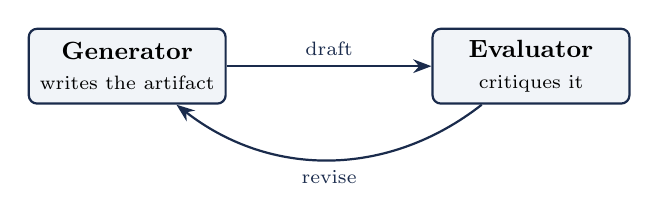
\begin{tikzpicture}[node distance=1.5cm, >=Stealth,
   box/.style={draw=navymain, thick, rounded corners=3pt, fill=navylight!25,
               minimum width=2.5cm, minimum height=0.95cm, align=center, font=\small}]
  \node[box] (gen) {\textbf{Generator}\\{\scriptsize writes the artifact}};
  \node[box, right=2.6cm of gen] (ev) {\textbf{Evaluator}\\{\scriptsize critiques it}};
  \draw[->, thick, navymain] (gen) -- node[above, font=\scriptsize] {draft} (ev);
  \draw[->, thick, navymain] (ev) to[bend left=38] node[below, font=\scriptsize] {revise} (gen);
\end{tikzpicture}

\vspace{0.5em}
\begin{flushleft}
\small
Anthropic's agent-harness post: put a \hl{generator} in a loop with an \hl{evaluator},
and the artifact keeps getting better --- for roughly ten rounds.
\cit{Anthropic, ``Building agent harnesses''}

\vspace{0.6em}
I reproduced this, and it does work:
\end{flushleft}

\vspace{-0.2em}
\begin{columns}[c,onlytextwidth]
\begin{column}{0.42\textwidth}\centering
  
\includegraphics[width=\linewidth]{img/demo_r0.png}\\
  {\scriptsize round 0 \quad\color{accentred}\textbf{4.5}}
\end{column}
\begin{column}{0.06\textwidth}\centering $\rightarrow$ \end{column}
\begin{column}{0.42\textwidth}\centering
  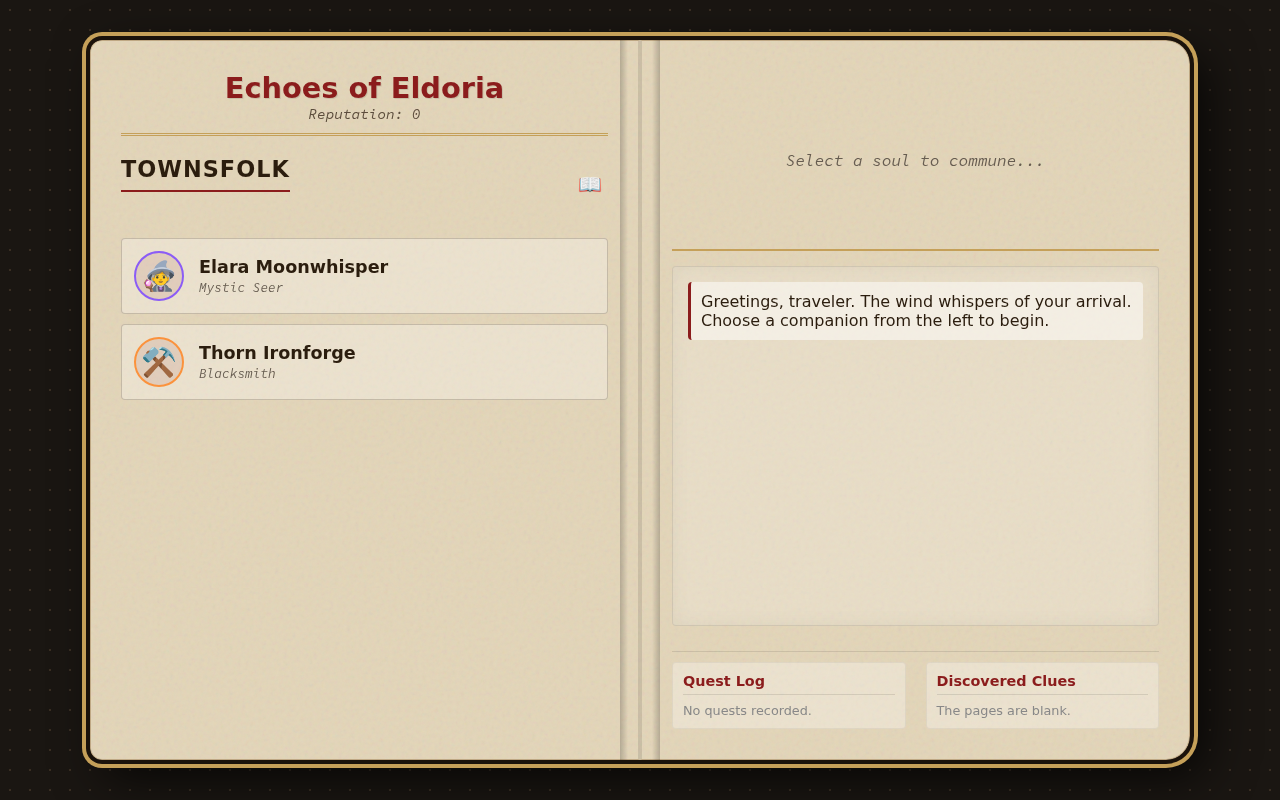
\includegraphics[width=\linewidth]{img/demo_mad.png}\\
  {\scriptsize after the loop \quad\color{winner}\textbf{7.8}}
\end{column}
\end{columns}

\vspace{0.4em}
\centering
{\small But the evaluator is \bad{one agent giving one verdict}. Should it be?}
\end{frame}

% ============================================ 2. MAD is contested
\begin{frame}{Multi-agent debate: promising, but contested}
\small
\begin{columns}[T,onlytextwidth]
\begin{column}{0.48\textwidth}
\begin{block}{\small The promise}
Several LLMs critique each other, then converge ---
better factuality and reasoning than one model alone.
\cit{Du+ '23; Liang+ '23}
\end{block}
\end{column}
\begin{column}{0.48\textwidth}
\begin{block}{\small The pushback}
Compute-matched, debate often \bad{fails to beat a single agent}
with good prompting / self-consistency.
\cit{Smit+ ICML'24, ``Should we be going MAD?''; Wang+ ACL'24}
\end{block}
\end{column}
\end{columns}

\vspace{0.8em}
\centering
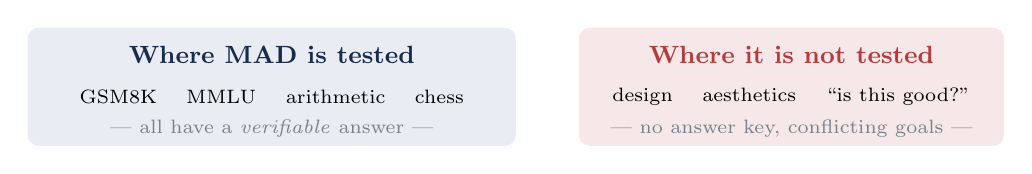
\begin{tikzpicture}[font=\scriptsize]
  \fill[navylight!40, rounded corners=4pt] (0,0) rectangle (6.2,1.5);
  \node[align=center, font=\small\bfseries, text=navymain] at (3.1,1.15) {Where MAD is tested};
  \node[align=center] at (3.1,0.62) {GSM8K \quad MMLU \quad arithmetic \quad chess};
  \node[align=center, text=gray60] at (3.1,0.22) {— all have a \emph{verifiable} answer —};

  \fill[accentred!12, rounded corners=4pt] (7.0,0) rectangle (12.4,1.5);
  \node[align=center, font=\small\bfseries, text=accentred] at (9.7,1.15) {Where it is not tested};
  \node[align=center] at (9.7,0.62) {design \quad aesthetics \quad ``is this good?''};
  \node[align=center, text=gray60] at (9.7,0.22) {— no answer key, conflicting goals —};
\end{tikzpicture}

\vspace{0.7em}
\centering
{\small MAD lives almost entirely in \hl{reasoning}, and \emph{there} its value is being questioned.}
\end{frame}

% ============================================ 3. The idea
\begin{frame}{The idea: point it at subjective quality instead}
\small
Subjective quality is currently improved by \hl{training-time preference learning}
--- RLHF, preference tuning, reward models. Expensive, and the reward is one scalar.
\cit{Ouyang+ '22; Bai+ '22}

\vspace{0.5em}
But ``good design'' is not one number --- it is \hl{several objectives that fight each other}:

\vspace{0.4em}
\centering
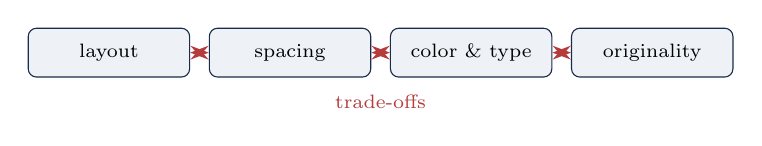
\begin{tikzpicture}[font=\scriptsize, >=Stealth,
  ax/.style={draw=navymain, rounded corners=3pt, fill=navylight!30,
             minimum width=2.05cm, minimum height=0.62cm, align=center}]
  \node[ax] (a) at (0,0)    {layout};
  \node[ax] (b) at (2.3,0)  {spacing};
  \node[ax] (c) at (4.6,0)  {color \& type};
  \node[ax] (d) at (6.9,0)  {originality};
  \draw[<->, accentred, thick] (a) -- (b);
  \draw[<->, accentred, thick] (b) -- (c);
  \draw[<->, accentred, thick] (c) -- (d);
  \node[text=accentred, font=\scriptsize] at (3.45,-0.62) {trade-offs};
\end{tikzpicture}

\vspace{0.6em}
\begin{columns}[c,onlytextwidth]
\begin{column}{0.44\textwidth}\centering
\textbf{\color{accentred}Today}\\[0.3em]
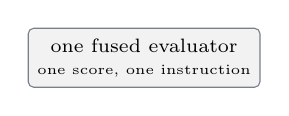
\begin{tikzpicture}[font=\scriptsize,
   b/.style={draw=gray60, rounded corners=2pt, fill=black!5, minimum width=2.7cm, minimum height=0.75cm, align=center}]
  \node[b] {one fused evaluator\\{\tiny one score, one instruction}};
\end{tikzpicture}
\end{column}
\begin{column}{0.1\textwidth}\centering $\Rightarrow$\end{column}
\begin{column}{0.44\textwidth}\centering
\textbf{\color{winner}This work}\\[0.3em]
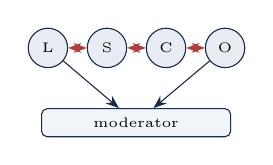
\begin{tikzpicture}[font=\tiny, >=Stealth,
   c/.style={draw=navymain, circle, fill=navylight!40, minimum size=0.5cm, inner sep=1pt}]
  \node[c] (c1) at (0,0.45) {L}; \node[c] (c2) at (0.75,0.45) {S};
  \node[c] (c3) at (1.5,0.45) {C}; \node[c] (c4) at (2.25,0.45) {O};
  \draw[<->, accentred] (c1)--(c2); \draw[<->, accentred] (c2)--(c3); \draw[<->, accentred] (c3)--(c4);
  \node[draw=navymain, rounded corners=2pt, fill=navylight!25, minimum width=2.4cm] (m) at (1.12,-0.5) {moderator};
  \draw[->, navymain] (c1) -- (m); \draw[->, navymain] (c4) -- (m);
\end{tikzpicture}\\[0.2em]
{\tiny one critic per objective, they argue, then synthesise}
\end{column}
\end{columns}

\vspace{0.7em}
\centering
\begin{block}{\small Research question}
\centering Can multi-agent debate raise \hl{subjective artifact quality} at \hl{inference time} ---
the setting it was never tested in, and where a single scalar reward fits worst?
\end{block}
\end{frame}

% ============================================ 4. What I am doing
\begin{frame}{What I am running}
\small
Same generator, same starting draft, same token budget --- \hl{only the evaluator changes}:

\vspace{0.5em}
\centering
\begin{tikzpicture}[font=\scriptsize, >=Stealth,
  s/.style={draw=navymain, thick, rounded corners=3pt, minimum width=2.5cm,
            minimum height=1.4cm, align=center, fill=navylight!20}]
  \node[s] (a) at (0,0)     {\textbf{SELF}\\[0.2em]{\tiny critiques\\ its own work}};
  \node[s] (b) at (3.0,0)   {\textbf{FUSED}\\[0.2em]{\tiny one evaluator\\ (the harness)}};
  \node[s] (c) at (6.0,0)   {\textbf{AXES}\\[0.2em]{\tiny one critic\\ per objective}};
  \node[s] (d) at (9.0,0)   {\textbf{MAD}\\[0.2em]{\tiny + they debate\\ each other}};
  \draw[->, gray60, thick] (a)--(b); \draw[->, gray60, thick] (b)--(c); \draw[->, gray60, thick] (c)--(d);
  \node[text=gray60, font=\tiny] at (4.5,-1.05) {more structure in the evaluator $\longrightarrow$};
\end{tikzpicture}

\vspace{0.8em}
\begin{columns}[T,onlytextwidth]
\begin{column}{0.48\textwidth}
\textbf{\color{navymain}Setup}
\begin{itemize}\itemsep0.15em
  \item 12 web-artifact tasks (ArtifactsBench)
  \item critics write \emph{critique only}; the generator rewrites the code
  \item judged by a \hl{held-out model}, \hl{blind}
        {\scriptsize (anonymised, shuffled, un-mapped after scoring)}
\end{itemize}
\end{column}
\begin{column}{0.48\textwidth}
\textbf{\color{navymain}Where it stands}
\begin{itemize}\itemsep0.15em
  \item Structured critics \gd{beat} the fused evaluator
        {\scriptsize (5.9 vs 5.4 out of 10)}
  \item But on \emph{pure} design tasks the gap \bad{disappears}
  \item An \emph{oracle} critic (aligned with the judge) lifts one round,
        then \bad{plateaus} --- so the bottleneck may be the generator, not the critique
\end{itemize}
\end{column}
\end{columns}

\vspace{0.6em}
\centering
{\small\color{gray60} Next: what kind of feedback actually survives revision.}
\end{frame}

\end{document}
